\subsection*{ГЛ13 1}
Возьмем случайную точку $A$ на конике и проведем прямые через нее и $P_1,P_2,P_3,P_4$ чтобы потом найти двойное отношение получченных прямых
\begin{figure}[h]
	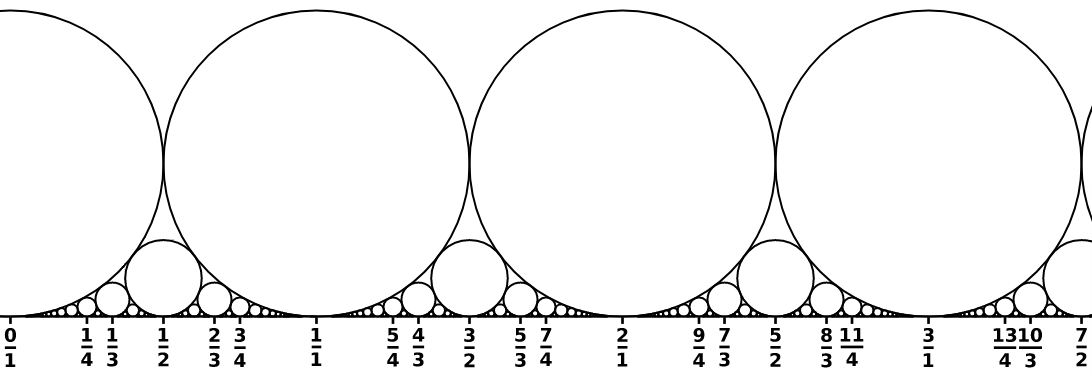
\includegraphics[width=0.35\linewidth]{pic5}
\end{figure}
Вспомним что при проективном преобразовании двойное отношение не меняется
\begin{figure}[h]
	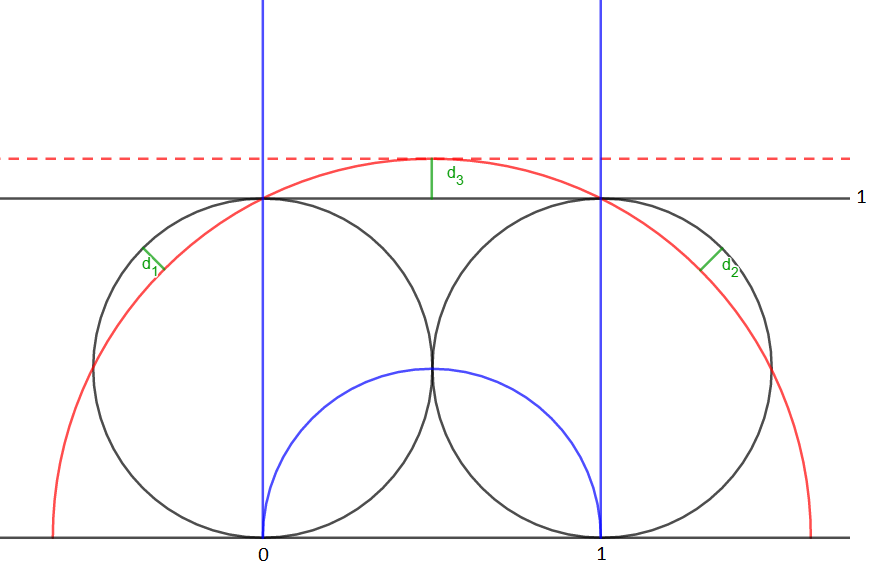
\includegraphics[width=0.35\linewidth]{pic6}
\end{figure}
Тогда заметим что $\sin((AP_1,AP_3)) = \sin((P_5P_1,P_5P_3))$ так как $\sin(x) = \sin(\pi - x)$, следовательно и двойные отношения 
\begin{gather*}
	\frac{\sin((P_5P_1,P_5P_3))}{\sin((P_5P_2,P_5P_3))} : \frac{\sin((P_5P_1,P_5P_4))}{\sin((P_5P_2,P_5P_4))}\\
	\frac{\sin((AP_1,AP_3))}{\sin((AP_2,AP_3))} : \frac{\sin((AP_1,AP_4))}{\sin((AP_2,AP_4))}
\end{gather*}
Равны, так как какую бы четверку точек на данной окружности мы ни рассмотрели, все они будут лежать на одной кружности, а $A$ и $P_5$ будут противоположными вершинами, из-за чего будут либо равны, либо в сумме давать $\pi$. Так как $A$ выбиралась случайнмобразом, то это двойное отношение равно для всех точек на конике, а вне коники оно будет иным(так как при переводе коники в окружность, точки лежащие вне нее там и остаются, то есть после преобразования точка будет вне окружноти и двойное отношение у нее будет иным)
		